\section{Syntax \& Aufbau eines \LaTeX -Dokuments}
 \begin{frame}
 	\frametitle{Inhalt}
 	\tableofcontents[%
 		currentsection, % causes all sections but the current to be shown in a semi-transparent way.
% % 		currentsubsection, % causes all subsections but the current subsection in the current section to ...
% % 		hideallsubsections, % causes all subsections to be hidden.
% 		hideothersubsections, % causes the subsections of sections other than the current one to be hidden.
% % 		part=, % part number causes the table of contents of part part number to be shown
% 		pausesections, % causes a \pause command to be issued before each section. This is useful if you
% 		pausesubsections, %  causes a \pause command to be issued before each subsection.
% % 		sections={ overlay specification },
 	]
 \end{frame}
\begin{frame}{Generelle Syntax}
	\begin{itemize}[<+->]
		\item alle Kommandos beginnen mit einem $\backslash$
		\item Kommentare mit einem \%
		\item Umgebungen beginnen mit $\backslash$begin\{ Umgebungsname\} und enden mit $\backslash$end\{Umgebungsname\}
	\end{itemize}
\end{frame}

\begin{frame}[fragile]{Beispiel Code}
	\lstsettex
	\begin{Code}
	\centering
		\begin{minipage}{0.9\textwidth}
	
		\lstinputlisting[linerange=1-19,title=\lstname]{./listings/demonstration.tex}
	
		\end{minipage}
	\end{Code}

\end{frame}
\begin{frame}[fragile]{Beispiel Code}
	\lstsettex
	\begin{Code}
	\centering
		\begin{minipage}{0.9\textwidth}
		\lstinputlisting[linerange=21-35,firstnumber=20,title=\lstname]{./listings/demonstration.tex}
		\end{minipage}
	\end{Code}

\end{frame}

\begin{frame}{Beispiel Ergebnis}
	\begin{figure}[tbph]
	\centering
	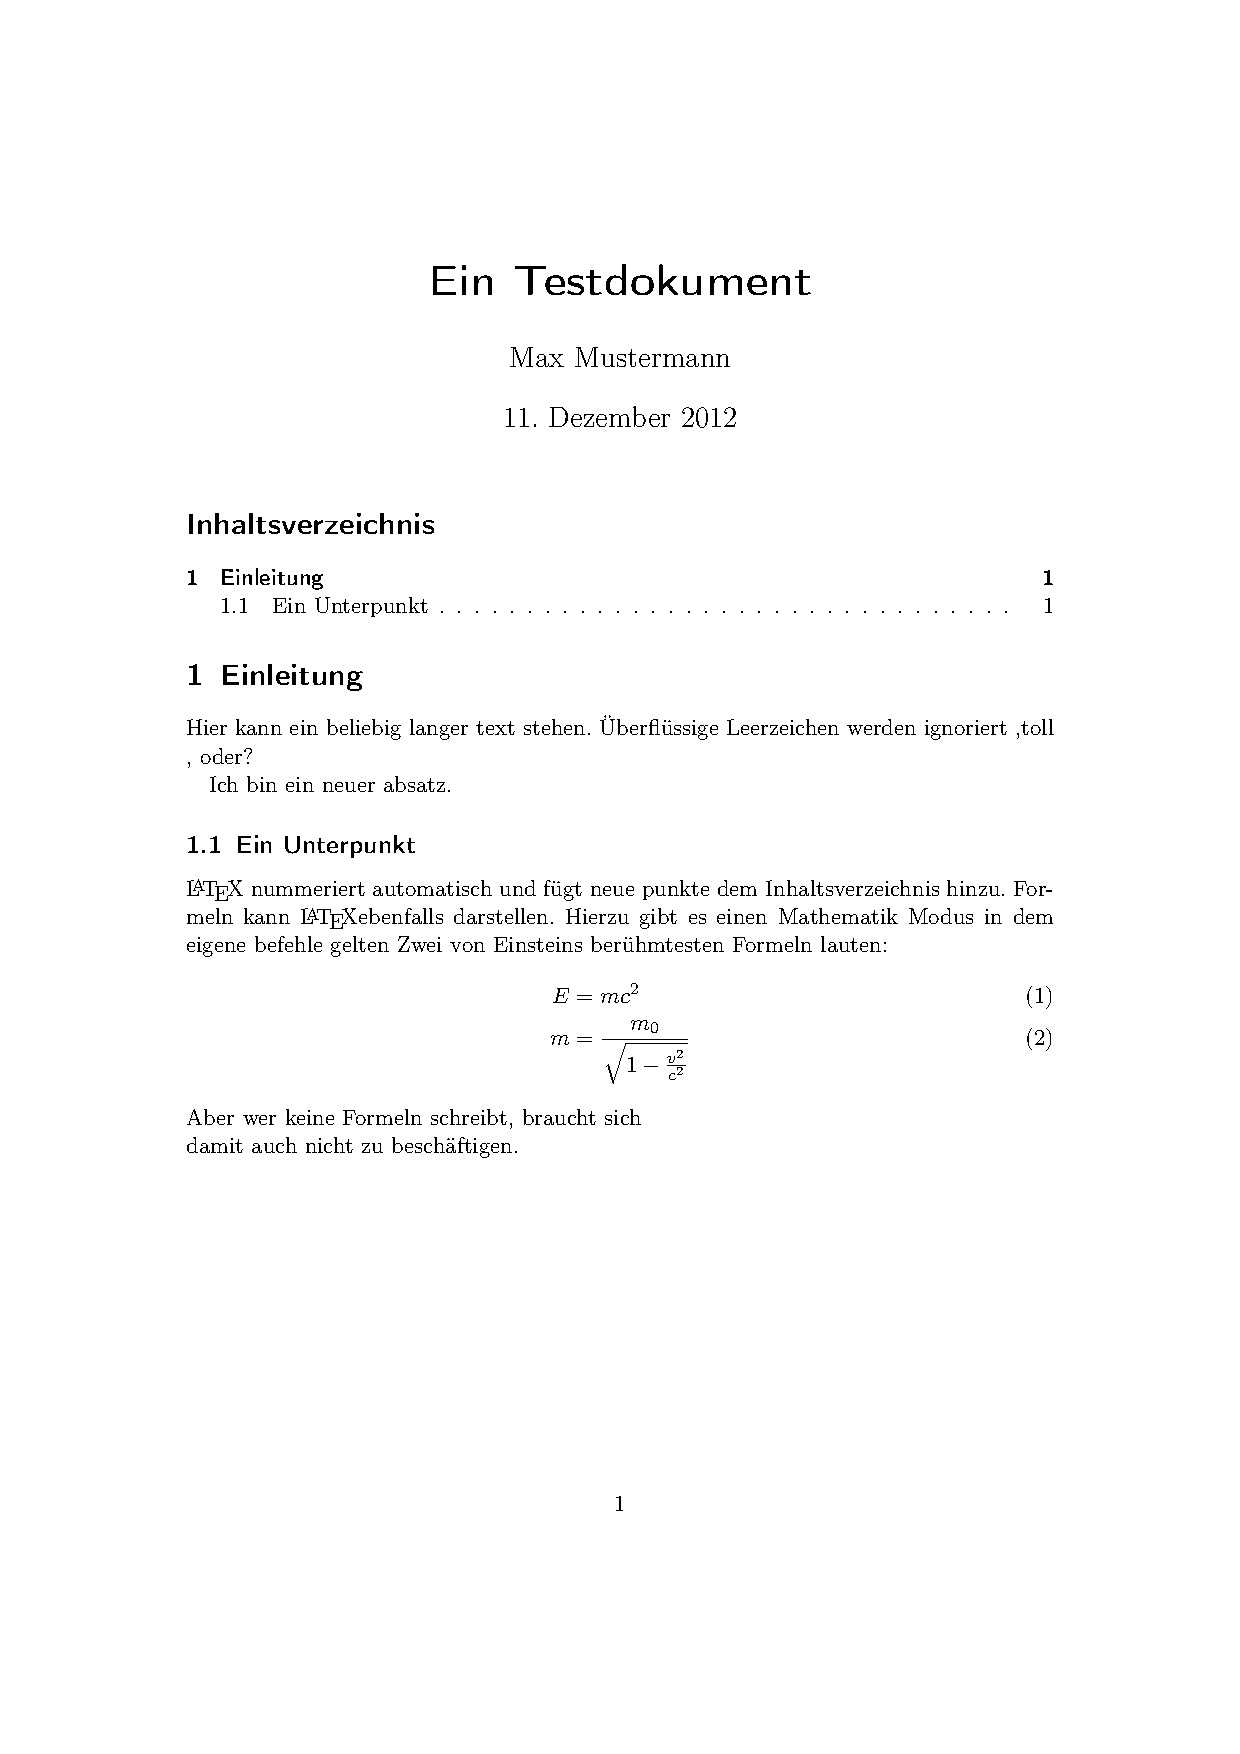
\includegraphics[height=\textheight]{./pictures/demonstration}
	\caption{Das PDF}
	\label{fig:demonstration}
	\end{figure}
\end{frame}

\begin{frame}{wichtige Befehle}
	\begin{itemize}[<+->]
	\item \lstinputlisting[linerange=1-1]{./listings/commands.tex} $ \Rightarrow $ \textbf{fett}
	\item \lstinputlisting[linerange=2-2]{./listings/commands.tex} $ \Rightarrow $ \textit{kursiv}
	\item \lstinputlisting[linerange=3-3]{./listings/commands.tex} $ \Rightarrow $ \underline{unterstrichen}
	\item \lstinputlisting[linerange=4-4]{./listings/commands.tex} $ \Rightarrow $ \textbf{\textit{\underline{kombination}}}
	\end{itemize}
\end{frame}